\documentclass{beamer}
\usetheme{Madrid}

\usepackage{graphicx}

\title{An Economic Analysis of Optimal Investment Strategies for Accumulating Housing Down Payments Among Generation Z in the United States}
\author{Frank Paul Longo II}
\date{\today}

\begin{document}

\frame{\titlepage}

\begin{frame}{Introduction}
    \begin{itemize}
        \item \textbf{Objective:} Identify optimal investment strategies for Generation Z to accumulate housing down payments.
        \item \textbf{Focus:} Practical solutions for achieving financial stability and homeownership.
    \end{itemize}
    \centering
    
\includegraphics[width=0.5\textwidth]{/Users/frank/Desktop/Project/Slides/Images/introduction_image.jpg}
\end{frame}

\begin{frame}{Why This Study Matters}
    \begin{itemize}
        \item \textbf{Financial Milestone:} Homeownership is a key goal for financial stability.
        \item \textbf{Challenges:} Generation Z faces unique challenges such as high student debt, rising living costs, and inflation.
        \item \textbf{Goal:} Provide practical investment strategies to overcome these challenges.
    \end{itemize}
    \centering
    
\includegraphics[width=0.5\textwidth]{/Users/frank/Desktop/Project/Slides/Images/why_this_study_matters.jpg}
\end{frame}

\begin{frame}{Background on Generation Z}
    \begin{itemize}
        \item \textbf{Born:} Between 1997 and 2012.
        \item \textbf{Characteristics:} Digital natives, socially conscious, and financially aware.
        \item \textbf{Financial Habits:} High value on financial security, but burdened with debt.
    \end{itemize}
    \centering
    
\includegraphics[width=0.5\textwidth]{/Users/frank/Desktop/Project/Slides/Images/gen_z_background.jpg}
\end{frame}

\begin{frame}{Financial Challenges}
    \begin{itemize}
        \item \textbf{Student Debt:} Average debt load for graduates is significant.
        \item \textbf{Living Costs:} Rent, utilities, and daily expenses are rising.
        \item \textbf{Inflation:} Erodes purchasing power and savings.
    \end{itemize}
    \centering
    
\includegraphics[width=0.5\textwidth]{/Users/frank/Desktop/Project/Slides/Images/financial_challenges.jpg}
\end{frame}

\begin{frame}{Homeownership Aspirations}
    \begin{itemize}
        \item \textbf{Financial Security:} Owning a home is a key step towards financial stability.
        \item \textbf{Investment:} Property can appreciate in value over time.
        \item \textbf{Independence:} Provides a sense of independence and accomplishment.
    \end{itemize}
    \centering
    
\includegraphics[width=0.5\textwidth]{/Users/frank/Desktop/Project/Slides/Images/homeownership_aspirations.jpg}
\end{frame}

\begin{frame}{Data Sources}
    \begin{itemize}
        \item \textbf{YFinance:} Financial data for stock and investment analysis.
        \item \textbf{FRED:} Economic data including inflation, interest rates, and unemployment.
    \end{itemize}
    \centering
    
\includegraphics[width=0.5\textwidth]{/Users/frank/Desktop/Project/Slides/Images/data_sources.jpg}
\end{frame}

\begin{frame}{Investment Strategies}
    \begin{itemize}
        \item \textbf{Conservative:} Focus on low-risk investments like bonds.
        \item \textbf{Balanced:} Mix of stocks and bonds to balance risk and return.
        \item \textbf{Aggressive:} High-risk, high-reward investments like equities.
    \end{itemize}
    \centering
    
\includegraphics[width=0.5\textwidth]{/Users/frank/Desktop/Project/Slides/Images/investment_strategies.jpg}
\end{frame}

\begin{frame}{Quantitative Approaches by Edward Thorp}
    \begin{itemize}
        \item \textbf{Pioneer in Quantitative Finance:} Developed methods to gain a financial edge.
        \item \textbf{Card Counting:} Applied in blackjack to improve odds.
        \item \textbf{Statistical Arbitrage:} Using statistical models to predict price movements.
    \end{itemize}
    \centering
    
\includegraphics[width=0.5\textwidth]{/Users/frank/Desktop/Project/Slides/Images/edward_thorp.jpg}
\end{frame}

\begin{frame}{Economic Variables}
    \begin{itemize}
        \item \textbf{Inflation:} General increase in prices, reducing purchasing power.
        \item \textbf{Interest Rates:} Cost of borrowing money, affects investment returns.
        \item \textbf{Unemployment Rates:} Percentage of the labor force that is jobless, affects economic stability.
    \end{itemize}
    \centering
    
\includegraphics[width=0.5\textwidth]{/Users/frank/Desktop/Project/Slides/Images/economic_variables.jpg}
\end{frame}

\begin{frame}{Behavioral Economics}
    \begin{itemize}
        \item \textbf{Psychological Factors:} Influence economic decisions.
        \item \textbf{Generation Z Traits:} Tech-savvy, risk-averse, and value-driven.
        \item \textbf{Financial Habits:} Impact of peer influence and social media on spending and saving.
    \end{itemize}
    \centering
    
\includegraphics[width=0.5\textwidth]{/Users/frank/Desktop/Project/Slides/Images/behavioral_economics.jpg}
\end{frame}

\begin{frame}{Modern Portfolio Theory (MPT)}
    \begin{itemize}
        \item \textbf{Diversification:} Spreading investments to reduce risk.
        \item \textbf{Efficient Frontier:} Optimal portfolios offering the highest return for a given risk level.
        \item \textbf{Capital Market Line:} Represents risk-return trade-offs.
    \end{itemize}
    \centering
    
\includegraphics[width=0.5\textwidth]{/Users/frank/Desktop/Project/Slides/Images/mpt.jpg}
\end{frame}

\begin{frame}{Home Costs and Down Payment Analysis}
    \begin{itemize}
        \item \textbf{Historical Trends:} Analysis of past housing prices.
        \item \textbf{Regional Differences:} Variation in home costs across regions.
        \item \textbf{Down Payment Impact:} How different down payment percentages affect loan costs.
    \end{itemize}
    \centering
    
\includegraphics[width=0.5\textwidth]{/Users/frank/Desktop/Project/Slides/Images/home_costs.jpg}
\end{frame}

\begin{frame}{Methodology}
    \begin{itemize}
        \item \textbf{Data Collection:} Economic data from FRED, behavioral data through surveys.
        \item \textbf{Simulation Models:} Monte Carlo simulations, Markov Chain Monte Carlo.
        \item \textbf{Analytical Techniques:} Gradient descent, linear algebra, risk-return analysis, life-cycle investing principles.
    \end{itemize}
    \centering
    
\includegraphics[width=0.5\textwidth]{/Users/frank/Desktop/Project/Slides/Images/methodology.jpg}
\end{frame}

\begin{frame}{Monte Carlo Simulations}
    \begin{itemize}
        \item \textbf{Purpose:} Generate probability distributions of achieving target down payment amounts.
        \item \textbf{Parameters:} Varying market conditions, economic factors.
        \item \textbf{Example:} Simulating future investment scenarios with different economic conditions.
    \end{itemize}
    \centering
    
\includegraphics[width=0.5\textwidth]{/Users/frank/Desktop/Project/Slides/Images/monte_carlo_simulations.jpg}
\end{frame}

\begin{frame}{Markov Chain Monte Carlo}
    \begin{itemize}
        \item \textbf{Purpose:} Model the stochastic processes underlying investment returns.
        \item \textbf{Advantages:} Improved accuracy in complex models.
        \item \textbf{Example:} Generating samples from the probability distribution by constructing a Markov chain.
    \end{itemize}
    \centering
    
\includegraphics[width=0.5\textwidth]{/Users/frank/Desktop/Project/Slides/Images/markov_chain_monte_carlo.jpg}
\end{frame}

\begin{frame}{Sensitivity Analysis}
    \begin{itemize}
        \item \textbf{Purpose:} Determine how different values of an independent variable affect a particular dependent variable.
        \item \textbf{Techniques:} Varying parameters to see changes in results.
        \item \textbf{Example:} Sensitivity of down payment accumulation to interest rate changes.
    \end{itemize}
    \centering
    
\includegraphics[width=0.5\textwidth]{/Users/frank/Desktop/Project/Slides/Images/sensitivity_analysis.jpg}
\end{frame}

\begin{frame}{Gradient Descent}
    \begin{itemize}
        \item \textbf{Purpose:} Optimize investment strategies by minimizing a cost function.
        \item \textbf{Application:} Finding the optimal asset allocation.
        \item \textbf{Example:} Using gradient descent to optimize the parameters of an investment model.
    \end{itemize}
    \centering
    
\includegraphics[width=0.5\textwidth]{/Users/frank/Desktop/Project/Slides/Images/gradient_descent.jpg}
\end{frame}

\begin{frame}{Linear Algebra}
    \begin{itemize}
        \item \textbf{Purpose:} Solve portfolio allocation problems.
        \item \textbf{Application:} Matrix operations for asset returns and risks.
        \item \textbf{Example:} Calculating the covariance matrix of asset returns.
    \end{itemize}
    \centering
    
\includegraphics[width=0.5\textwidth]{/Users/frank/Desktop/Project/Slides/Images/linear_algebra.jpg}
\end{frame}

\begin{frame}{Risk-Return Analysis}
    \begin{itemize}
        \item \textbf{Purpose:} Assess the trade-off between risk and expected return.
        \item \textbf{Techniques:} Sharpe ratio, volatility measures.
        \item \textbf{Example:} Comparing the risk-return profiles of different investment portfolios.
    \end{itemize}
    \centering
    
\includegraphics[width=0.5\textwidth]{/Users/frank/Desktop/Project/Slides/Images/risk_return_analysis.jpg}
\end{frame}

\begin{frame}{Lifecycle Investing}
    \begin{itemize}
        \item \textbf{Purpose:} Adjust risk exposure as individuals approach their home purchase date.
        \item \textbf{Strategies:} Gradual shift from high-risk to low-risk investments.
        \item \textbf{Example:} Dynamic asset allocation based on time horizon.
    \end{itemize}
    \centering
    
\includegraphics[width=0.5\textwidth]{/Users/frank/Desktop/Project/Slides/Images/lifecycle_investing.jpg}
\end{frame}

\begin{frame}{Simulation Outcomes}
    \begin{itemize}
        \item \textbf{Results:} Probability distributions of achieving target down payment amounts.
        \item \textbf{Insights:} Impact of different investment strategies and economic variables.
        \item \textbf{Recommendations:} Optimal strategies for Generation Z based on simulation outcomes.
    \end{itemize}
    \centering
    
\includegraphics[width=0.5\textwidth]{/Users/frank/Desktop/Project/Slides/Images/simulation_outcomes.jpg}
\end{frame}

\begin{frame}{Economic Impact}
    \begin{itemize}
        \item \textbf{Implications:} How investment strategies affect the broader economy.
        \item \textbf{Policy Recommendations:} Suggestions for economic policies to support Generation Z.
        \item \textbf{Future Research:} Areas for further study and analysis.
    \end{itemize}
    \centering
    
\includegraphics[width=0.5\textwidth]{/Users/frank/Desktop/Project/Slides/Images/economic_impact.jpg}
\end{frame}

\begin{frame}{Optimized Asset Allocation}
    \begin{itemize}
        \item \textbf{Purpose:} Determine the best mix of assets for down payment savings.
        \item \textbf{Techniques:} Modern Portfolio Theory, lifecycle investing.
        \item \textbf{Example:} Optimal asset allocation for a young professional saving for a home.
    \end{itemize}
    \centering
    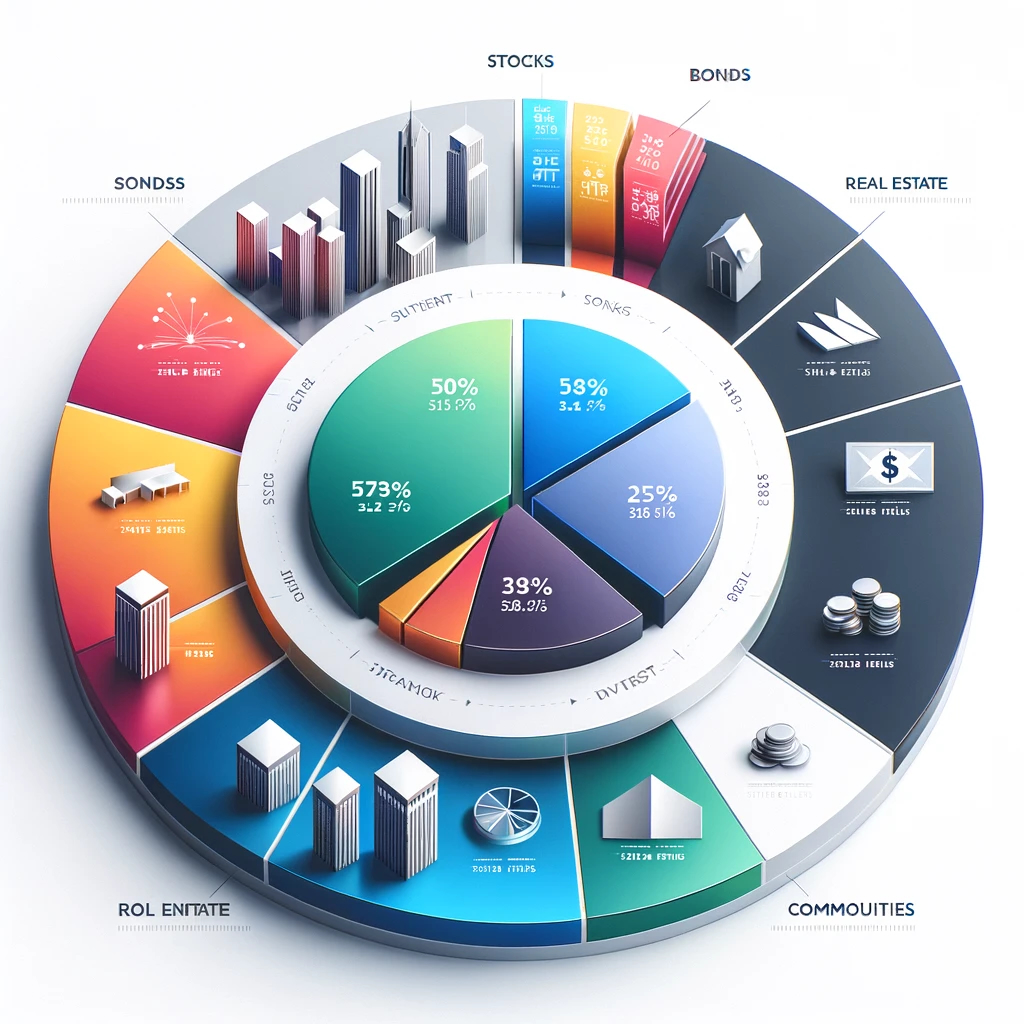
\includegraphics[width=0.5\textwidth]{/Users/frank/Desktop/Project/Slides/Images/asset_allocation.jpg}
\end{frame}

\begin{frame}{Behavioral Insights}
    \begin{itemize}
        \item \textbf{Purpose:} Understand how Generation Z’s behavior affects their investment decisions.
        \item \textbf{Techniques:} Behavioral finance principles, surveys.
        \item \textbf{Example:} Impact of social media on saving and spending habits.
    \end{itemize}
    \centering
    
\includegraphics[width=0.5\textwidth]{/Users/frank/Desktop/Project/Slides/Images/behavioral_insights.jpg}
\end{frame}

\begin{frame}{Down Payment Accumulation}
    \begin{itemize}
        \item \textbf{Strategies:} Effective ways to save for a down payment.
        \item \textbf{Techniques:} Automatic savings, high-yield savings accounts, investing in REITs.
        \item \textbf{Example:} Using a combination of savings and investments to reach down payment goals.
    \end{itemize}
    \centering
    
\includegraphics[width=0.5\textwidth]{/Users/frank/Desktop/Project/Slides/Images/down_payment.jpg}
\end{frame}

\begin{frame}{Trends in Home Costs}
    \begin{itemize}
        \item \textbf{Historical Analysis:} Trends in housing prices over the last few decades.
        \item \textbf{Future Predictions:} Expected trends in housing costs.
        \item \textbf{Impact on Strategy:} How housing cost trends affect investment strategies.
    \end{itemize}
    \centering
    
\includegraphics[width=0.5\textwidth]{/Users/frank/Desktop/Project/Slides/Images/home_cost_trends.jpg}
\end{frame}

\begin{frame}{Conclusion}
    \begin{itemize}
        \item \textbf{Summary:} Recap of findings and recommendations.
        \item \textbf{Next Steps:} Future research and practical applications.
        \item \textbf{Acknowledgements:} Thanking contributors and supporters.
    \end{itemize}
    \centering
    
\includegraphics[width=0.5\textwidth]{/Users/frank/Desktop/Project/Slides/Images/conclusion.jpg}
\end{frame}

\begin{frame}{Q&A}
    \begin{itemize}
        \item \textbf{Discussion:} Open floor for questions and discussions.
        \item \textbf{Clarifications:} Address any uncertainties or elaborations needed.
    \end{itemize}
    \centering
    
\includegraphics[width=0.5\textwidth]{/Users/frank/Desktop/Project/Slides/Images/qa_image.jpg}
\end{frame}

\end{document}
